\documentclass[12pt]{article}
\usepackage{threeparttable}
\usepackage{booktabs}
\usepackage{inputenc, amsmath,amssymb, amsthm}
\usepackage[font=small,labelfont=bf,
   justification=justified,
   format=plain]{caption}
\usepackage{subcaption}
\usepackage{longtable}
\usepackage{adjustbox}
\usepackage{graphicx}
\newtheorem{theorem}{Theorem}
\usepackage{xcolor}
\usepackage{float}
\usepackage[colorlinks=true,
            linkcolor=blue,      % color of internal links (sections, pages, etc)
            citecolor=blue,      % color of citation links
            urlcolor=blue,       % color of URL links
            filecolor=blue]{hyperref}
\usepackage{url}
\usepackage{array}
\usepackage{url}
\usepackage{tikz}
\usetikzlibrary{shapes.geometric, arrows, positioning, fit}
\usetikzlibrary{calc}
\usepackage{titling}
\usepackage{lipsum}
\usepackage{natbib}
\usepackage{setspace}
\usepackage[margin=.75in]{geometry}
\usepackage{xcolor}
\usepackage{amsmath, amssymb, amsfonts}  % loads all AMS symbols & environments

\theoremstyle{definition}
\newtheorem{definition}{Definition}[section]
\usepackage[english]{babel}

\onehalfspacing


\graphicspath{{../../../../../Dropbox/Lawsuits Asymmetry/output}}


\title{Entitlement Pipeline: Data Cleaning}
\author{Tyler Jacobson}
\begin{document}
\maketitle
\section{To Do List}
\subsection{Descriptives}
Appeals
\begin{enumerate}
    \item What fraction of projects are appealed? 
    \item How long does the appeal take? 
    \item What fraction of appeals are granted?
    \item How does the location and size of the project affected whether the project gets appealed?
    \item Do appealed projects get built at the same rate as others?
\end{enumerate}
Lawsuits
\begin{enumerate}
    \item What fraction of projects are litigated? 
    \item How long does the lawsuit take? 
    \item What fraction of lawsuits are granted?
    \item How does the location and size of the project affected whether the project gets sued?
    \item Do litigated projects get built at the same rate as others?
\end{enumerate}
Combined:
\begin{enumerate}
    \item What is the cumulative amount of time an opponent could add to the project?
    \item How does the likelihood of completion depend on the amount of time in the planning process
\end{enumerate}
\subsection{Framework}
Key question: how costly is a delay? argument is that it depends greatly on project risk and the upfront level of investment firms must put into the process. With no upfront cost, then there is no real cost of delays, everything is proposed. How risky are projects? Can we say anything about that? Our best hope is to use a congestion instrument. 
\subsection{Congestion}

Approval timelines in the United States are long and variable. Opponents to new housing have tools at their disposal to extend timelines and make approval more difficult for developers. For example, in Los Angeles, anyone may appeal a city planning decision or choose to litigate the decision by arguing the review process did not properly follow environmental review. We find that these delay tactics are common with X\% housing units proposed between 2015 and 2025 facing one of these two tools. Comparing similar projects that were or were not sued/appealed, we find that these delays considerably reduce the probability that projects complete and break ground even if they are eventually approved. The dropout due to delay suggests using a high discount factor when predicting the effect of 


\section{Example}
DIR-2023-2838-TOC-SPP-SPR-HCA
Location 4627 W Hollywood
Filed on 4/24/2023
Approved 9/17/2024
Appealed on 9/23/2024: Planning application
LA CPC denied the appeal on 1/23/2025 (Important to know that this not what is in the data)
CEQA Appeal on 2/7/2025
City council rejects appeal on 6/5/2025
https://la.urbanize.city/post/la-city-council-upholds-approval-mixed-use-project-4627-hollywood-blvd
Appeals added roughly 9 months to the approval process and added an additional two vetos. 

Here is the appeal being \hyperlink{https://cityclerk.lacity.org/lacityclerkconnect/index.cfm?fa=ccfi.viewrecord&cfnumber=25-0201}{rejected}

\begin{figure}[H]
\centering
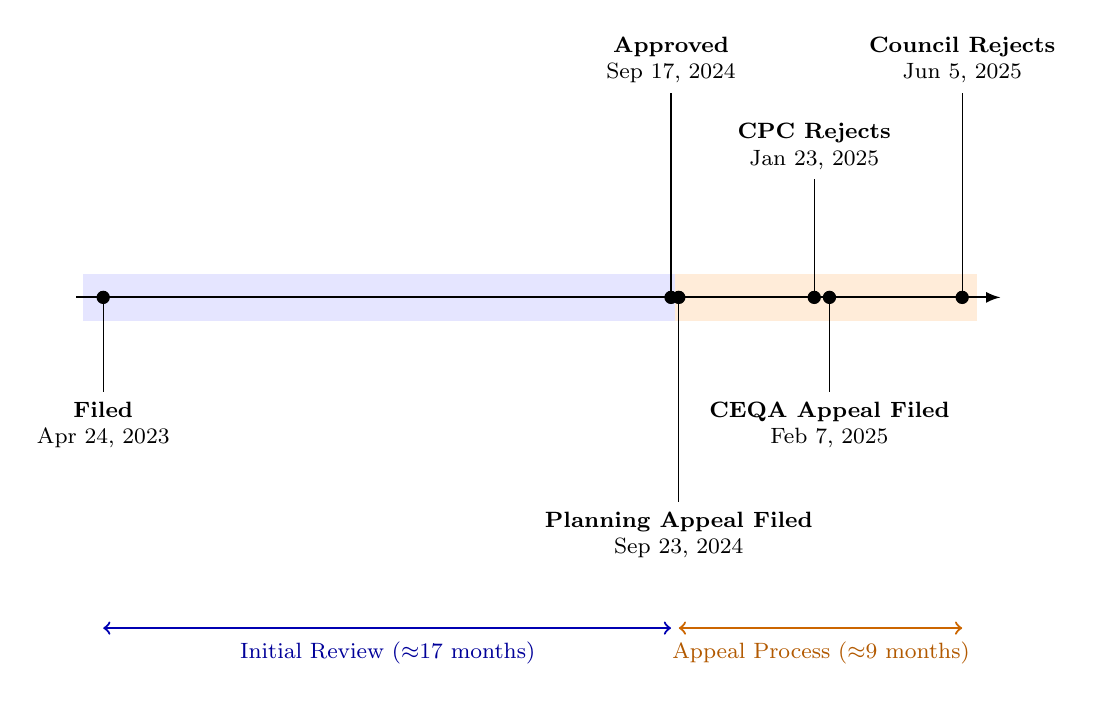
\begin{tikzpicture}[x=0.43cm, y=1cm, font=\footnotesize]

  % x positions in months from Apr 2023
  \def\xFiled{0}
  \def\xApproved{16.77}
  \def\xPlanAppeal{17.0}
  \def\xCPCDenied{21.0}
  \def\xCEQAAppeal{21.45}
  \def\xCouncil{25.37}

  % Phase shading
  \fill[blue!10]   (-0.6, -0.3) rectangle (16.9, 0.3);
  \fill[orange!15] (16.9, -0.3) rectangle (25.8, 0.3);

  % Main timeline axis
  \draw[thick, -latex] (-0.8, 0) -- (26.5, 0);

  % Event dots
  \foreach \x in {\xFiled, \xApproved, \xPlanAppeal, \xCPCDenied, \xCEQAAppeal, \xCouncil}
    \filldraw[black] (\x, 0) circle (2.2pt);

  % Filed (below)
  \draw[thin] (\xFiled, 0) -- (\xFiled, -1.2);
  \node[below, align=center] at (\xFiled, -1.2) {\textbf{Filed}\\Apr 24, 2023};

  % Approved (above, tall stem to clear Planning Appeal label)
  \draw[thin] (\xApproved, 0) -- (\xApproved, 2.6);
  \node[above, align=center] at (\xApproved, 2.6) {\textbf{Approved}\\Sep 17, 2024};

  % Planning Appeal (below, deep stem to clear Approved label)
  \draw[thin] (\xPlanAppeal, 0) -- (\xPlanAppeal, -2.6);
  \node[below, align=center] at (\xPlanAppeal, -2.6) {\textbf{Planning Appeal Filed}\\Sep 23, 2024};

  % CPC Denies (above)
  \draw[thin] (\xCPCDenied, 0) -- (\xCPCDenied, 1.5);
  \node[above, align=center] at (\xCPCDenied, 1.5) {\textbf{CPC Rejects}\\Jan 23, 2025};

  % CEQA Appeal (below)
  \draw[thin] (\xCEQAAppeal, 0) -- (\xCEQAAppeal, -1.2);
  \node[below, align=center] at (\xCEQAAppeal, -1.2) {\textbf{CEQA Appeal Filed}\\Feb 7, 2025};

  % City Council Rejects (above)
  \draw[thin] (\xCouncil, 0) -- (\xCouncil, 2.6);
  \node[above, align=center] at (\xCouncil, 2.6) {\textbf{Council Rejects}\\Jun 5, 2025};

  % Phase duration arrows
  \draw[<->, blue!70!black, thick] (\xFiled, -4.2) -- (\xApproved, -4.2);
  \node[below, blue!60!black, align=center] at (8.4, -4.25)
        {Initial Review ($\approx$17 months)};

  \draw[<->, orange!80!black, thick] (\xPlanAppeal, -4.2) -- (\xCouncil, -4.2);
  \node[below, orange!70!black, align=center] at (21.2, -4.25)
        {Appeal Process ($\approx$9 months)};

\end{tikzpicture}
\caption{Case timeline for DIR-2023-2838 (4627 W Hollywood Blvd). The planning appeal was filed six days after approval; appeals added roughly nine months to the overall process.}
\end{figure}

So according to my entitlements data, this was filed on 
4/24/2023 
completed on 
9/17/2024
Max app date:
17sep2024
Min filing date
24apr2023

So we are not getting the data right here. Data on appeals comes from both the city planning commission and from the city council. The CPC has minutes pdfs of varying quality 

\section{Comparing Appealed and Non-Appealed Projects}
Here I am restricting to projects that have unit counts. 

\begin{table}[H]
    \centering
    \input{../../../../../Dropbox/Lawsuits Asymmetry/output/appeals/sum_stats_appeals.tex}
\caption{Summary Stats}
\end{table}






\section{How Do Appeals Change When Projects Get Built?}
To see how appeals change when and whether projects get built, I run the following descriptive event study specification:
$$Y_{it}=\sum_{k\neq -1}\left(\tau_k B_{i,k} + \tau_k^A 1\{A_i = 1\} * B_{i,k}\right) +  \beta X_i  + \phi_t + \epsilon_{i,t}$$
where $Y_{it}$ is whether project $i$ is built (instanteously or cumulatively) in month $t$. $B_{i,k}$ is an indicator for the month relative to when the application was initially approved. $A_i$ is an indicator for whether application $i$ was appealed (at time $a$). $X_i$ are a set of controls (log units, log case length, and whether the project was appealed at all). $\phi_t$ are monthly fixed effects. By construction, there are no projects receiving building permits prior to getting approval. $\tau_k^A$ are the coefficients of interest, which can be read as the differential (cumulative or instantaneous) permitting rate of appealed projects, $k$ months after approval.  

\begin{figure}[H]
  \centering
  \begin{subfigure}[t]{0.48\textwidth}
    \centering
    \includegraphics[width=\textwidth]{appeals/event_study_match.pdf}
    \caption{Monthly Build Rates}
  \end{subfigure}
  \hfill
  \begin{subfigure}[t]{0.48\textwidth}
    \centering
    \includegraphics[width=\textwidth]{appeals/event_study_cum_match.pdf}
    \caption{Cumulative Build Rates}
  \end{subfigure}
  \caption{Effect of Appeals on Building Completion}
\end{figure}


\subsection{Which Projects are Likely to be Appealed?}






\end{document}